% Provenance (never printed): cycle 4 SVT, "La planete Terre": the history of
% the Earth read in the rocks, relative dating (superposition, recoupement,
% inclusion, continuite paleontologique), the ages of the Earth, eras and
% periods, the scale of geological time; see sources/book1/PROVENANCE.md.
% Book 1, grade 7, chapter 5.
% Vocabulary guard: owns relative dating / absolute age, the four principles,
% unconformity, era and geological period, the geological time scale. The
% method of radiometric dating is the physics books' and grade 12's: told
% here in two sentences, never defined. Fossils as evidence of evolution are
% the biology books' (one sentence of prose). "Ice age" is grade 8's: not used.
\chapter{De ouderdom van de Aarde}\label{ch:g7:geological-time}

In juni 1788 bezochten de Schotse geoloog James Hutton en twee vrienden,
de wiskundige John Playfair en de scheikundige James Hall, Siccar Point,
een rotsachtige landtong aan de \omterm{def:g1:landscapes-around-us:water}{kust} van Schotland, ``kaalgespoeld door
de \omterm{def:g2:water-on-earth:ocean}{zee}''. Onder aan de rots zagen ze grijze lagen die op hun kant stonden,
bijna verticaal. Daarboven lagen banken rood zandsteen, flauw hellend.
Hutton legde uit wat er was gebeurd: de grijze lagen waren vlak neergelegd
op de bodem van een \omterm{def:g2:water-on-earth:ocean}{zee}, daarna op hun kant geduwd en vervolgens
weggesleten, voordat het rode \omterm{def:g3:stones-pebbles-sand:sand}{zand} erbovenop werd gelegd. Elk van die
stappen had een onmetelijke tijd nodig. Playfair schreef later: ``De geest
leek duizelig te worden door zo ver in de afgrond van de tijd te kijken.''
% ledger: ncse:siccar-point

\begin{omfigure}
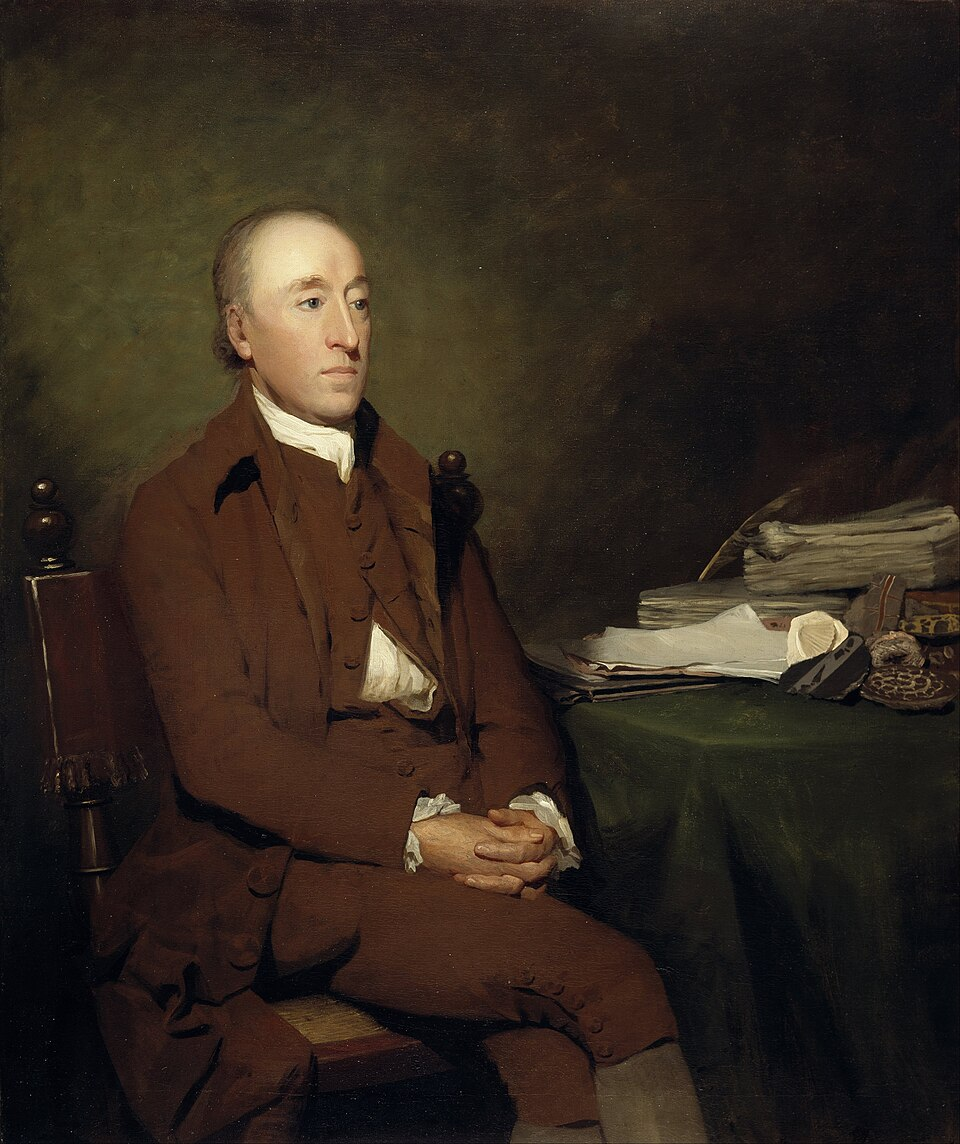
\includegraphics[width=0.3\linewidth]{images/book1/g7-hutton.jpg}

{\small James Hutton (1726--1797), geschilderd door Henry Raeburn. Hutton
zag elke laag als een tijdspanne, met de oudste onderaan overal waar de
lagen niet zijn omgekeerd. Portret in het publieke domein, via Wikimedia
Commons.}
% ledger: commons:hutton-portrait, usgs:hutton-smith
\label{fig:g7:geological-time:hutton}
\end{omfigure}

Hoe kunnen we zien welk \omterm{def:g3:stones-pebbles-sand:rock}{gesteente} ouder is dan een ander, zonder dat er
een datum op staat? Hoe oud is de Aarde? En hoe kun je je zo'n lange
geschiedenis eigenlijk voorstellen?

\begin{recall}
\omterm{def:g7:sediments-and-fossils:sediment}{Sedimenten} bezinken in lagen, de ene boven op de andere, en worden hard
tot \omterm{def:g6:rocks-and-minerals:rock-families}{afzettingsgesteente}; \omterm{def:g7:sediments-and-fossils:fossil}{fossielen} zijn de overblijfselen of sporen van
levende wezens, bewaard in \omterm{def:g3:stones-pebbles-sand:rock}{gesteente} (\cref{ch:g7:sediments-and-fossils}).
Een \emph{\omterm{def:g7:earthquakes:fault}{breuk}} is een scheur in het \omterm{def:g3:stones-pebbles-sand:rock}{gesteente} waarlangs de twee kanten
zijn verschoven (\cref{ch:g7:earthquakes}). Graniet is een
\emph{\omterm{def:g6:rocks-and-minerals:rock-families}{stollingsgesteente}}: het ontstaat als gesmolten \omterm{def:g3:stones-pebbles-sand:rock}{gesteente} diep onder
de grond langzaam afkoelt; schist is een \emph{\omterm{def:g6:rocks-and-minerals:rock-families}{metamorf gesteente}},
veranderd door hitte en druk; een conglomeraat is een \omterm{def:g6:rocks-and-minerals:rock-families}{afzettingsgesteente}
van aan elkaar gekitte \omterm{def:g3:stones-pebbles-sand:pebble}{kiezels} (\cref{ch:g6:rocks-and-minerals}).
\end{recall}

\section{Wat kwam eerst?}

Historici kunnen gebeurtenissen in volgorde zetten, zelfs zonder hun
datum. De Eerste Wereldoorlog kwam voor de Tweede: hun namen zeggen het al.
Er stond nog geen televisie in de huiskamers toen de gebroeders Wright in
1903 voor het eerst vlogen, maar veel mensen keken in 1969 op televisie naar
de eerste stappen op de Maan: dus kwam eerst de vlucht, dan de televisie in
huis, dan de Maan. Aanwijzingen verzamelen en vergelijken is genoeg om de
volgorde te vinden. Voor bijna de hele geschiedenis van de Aarde bestaat er
helemaal geen geschreven verslag, en geologen werken op dezelfde manier:
ze gebruiken aanwijzingen die in het \omterm{def:g3:stones-pebbles-sand:rock}{gesteente} bewaard zijn.
% ledger: usgs:events-order

\begin{definition}[Relatieve datering en absolute ouderdom]\label{def:g7:geological-time:relative-dating}
\emph{Relatieve datering}\index{relatieve datering} zet \omterm{def:g3:stones-pebbles-sand:rock}{gesteenten} en
gebeurtenissen in volgorde, van het oudste tot het jongste, zonder te zeggen
hoeveel jaar geleden ze plaatsvonden: dit \omterm{def:g3:stones-pebbles-sand:rock}{gesteente} is ouder dan dat. Een
\emph{absolute ouderdom}\index{absolute ouderdom} is een ouderdom die als
een aantal jaren wordt gegeven, bijvoorbeeld ``\num{300} miljoen jaar''.
\end{definition}

\section{Vier principes om gesteenten in volgorde te zetten}

Vier eenvoudige principes doen het meeste werk van de \omterm{def:g7:geological-time:relative-dating}{relatieve datering}.
Ze zijn hieronder afgebeeld, in vier denkbeeldige kliffen. Het eerste werd
in 1669 door Nicolaus Steno geformuleerd; Hutton bouwde er aan het eind van
de achttiende eeuw op voort.
% ledger: usgs:hutton-smith, og:stratigraphy-principles

\begin{omfigure}
\tikzset{
  trilo/.pic={\fill[black!65] (0,0) ellipse (0.13 and 0.085);
              \draw[white, line width=0.3pt] (-0.11,0.028) -- (0.11,0.028) (-0.11,-0.028) -- (0.11,-0.028);},
  ammo/.pic={\draw[black!75, line width=0.45pt] (0,0) circle (0.1) (0,0) circle (0.062) (0,0) circle (0.028);}
}
\begin{minipage}[t]{0.49\linewidth}\centering
\begin{tikzpicture}[font=\footnotesize]
  \fill[lith sandstone] (0,0) rectangle (4.4,0.6);
  \fill[lith shale] (0,0.6) rectangle (4.4,1.2);
  \fill[lith limestone] (0,1.2) rectangle (4.4,1.8);
  \fill[lith sandstone] (0,1.8) rectangle (4.4,2.4);
  \foreach \k in {1,2,3,4} \node[fill=white, inner sep=1pt] at (0.35,0.6*\k-0.3) {\k};
  \draw (0,0) rectangle (4.4,2.4);
  \foreach \y in {0.6,1.2,1.8} \draw[contact] (0,\y) -- (4.4,\y);
  \draw[-{Stealth}, line width=0.8pt] (4.75,0.1) -- (4.75,2.3);
  \node[anchor=west] at (4.85,2.2) {jongste};
  \node[anchor=west] at (4.85,0.2) {oudste};
\end{tikzpicture}

{\small (a) Superpositie: laag 1 ontstond eerst, laag 4 het laatst.}
\end{minipage}\hfill
\begin{minipage}[t]{0.49\linewidth}\centering
\begin{tikzpicture}[font=\footnotesize]
  % left block, below the fault
  \begin{scope}
    \clip (0,0) -- (3.75,0) -- (3.25,2.4) -- (0,2.4) -- cycle;
    \fill[lith sandstone] (0,0) rectangle (5,0.6);
    \fill[lith shale] (0,0.6) rectangle (5,1.2);
    \fill[lith limestone] (0,1.2) rectangle (5,1.8);
    \fill[lith granite] (1.2,0) -- (1.85,0) -- (1.75,0.9) -- (1.9,1.8) -- (1.15,1.8) -- (1.3,0.9) -- cycle;
    \fill[lith sandstone] (0,1.8) rectangle (5,2.4);
    \foreach \y in {0.6,1.2} {\draw[contact] (0,\y) -- (1.25,\y); \draw[contact] (1.8,\y) -- (5,\y);}
    \draw[contact] (1.2,0) -- (1.3,0.9) -- (1.15,1.8) (1.85,0) -- (1.75,0.9) -- (1.9,1.8);
    \draw[contact] (0,1.8) -- (5,1.8);
  \end{scope}
  % right block, moved down along the fault
  \begin{scope}
    \clip (3.75,0) -- (5,0) -- (5,2.05) -- (3.32,2.05) -- cycle;
    \fill[lith sandstone] (3,-0.35) rectangle (5,0.25);
    \fill[lith shale] (3,0.25) rectangle (5,0.85);
    \fill[lith limestone] (3,0.85) rectangle (5,1.45);
    \fill[lith sandstone] (3,1.45) rectangle (5,2.05);
    \foreach \y in {0.25,0.85,1.45} \draw[contact] (3,\y) -- (5,\y);
  \end{scope}
  \draw (0,0) -- (5,0) -- (5,2.05) -- (3.32,2.05) (3.25,2.4) -- (0,2.4) -- (0,0);
  \draw[fault] (3.75,0) -- (3.25,2.4);
  \node[anchor=south, fill=white, inner sep=1pt] at (1.5,2.45) {graniet};
  \draw[black!70] (1.5,2.45) -- (1.52,1.6);
  \node[anchor=south] at (4.2,2.45) {breuk};
  \draw[black!70] (4.0,2.45) -- (3.4,1.75);
\end{tikzpicture}

{\small (b) Doorsnijding: het graniet is jonger dan de drie lagen die het
doorsnijdt en ouder dan de bovenste laag; de \omterm{def:g7:earthquakes:fault}{breuk}, die ze allemaal breekt,
is het jongst.}
\end{minipage}

\bigskip
\begin{minipage}[t]{0.49\linewidth}\centering
\begin{tikzpicture}[font=\footnotesize]
  \fill[lith granite] (0,0) -- (4.4,0) -- (4.4,1.05) .. controls (3.4,0.95) and (2.6,1.2) .. (1.6,1.0) .. controls (0.9,0.88) and (0.4,1.1) .. (0,1.0) -- cycle;
  \fill[lith conglomerate] (0,2.4) -- (4.4,2.4) -- (4.4,1.05) .. controls (3.4,0.95) and (2.6,1.2) .. (1.6,1.0) .. controls (0.9,0.88) and (0.4,1.1) .. (0,1.0) -- cycle;
  \foreach \x/\y/\a/\b in {0.5/1.35/0.2/0.12, 1.3/1.25/0.16/0.1, 2.1/1.45/0.22/0.13, 2.9/1.3/0.17/0.11, 3.7/1.4/0.2/0.12, 0.9/1.8/0.15/0.1, 2.5/1.95/0.17/0.1, 3.4/1.85/0.14/0.09}
    \filldraw[fill=omLithGranite, draw=black!70, line width=0.3pt] (\x,\y) ellipse [x radius=\a, y radius=\b];
  \draw[unconformity] (0,1.0) .. controls (0.4,1.1) and (0.9,0.88) .. (1.6,1.0) .. controls (2.6,1.2) and (3.4,0.95) .. (4.4,1.05);
  \draw (0,0) rectangle (4.4,2.4);
  \node[fill=white, inner sep=1pt] at (2.2,0.45) {graniet};
  \node[anchor=west] at (4.5,1.7) {conglomeraat};
  \node[anchor=west, align=left] at (4.5,1.15) {kiezels van\\graniet};
  \draw[black!70] (4.5,1.15) -- (3.85,1.4);
\end{tikzpicture}

{\small (c) Insluiting: de \omterm{def:g3:stones-pebbles-sand:pebble}{kiezels} van graniet zijn ouder dan het
conglomeraat waarin ze zitten.}
\end{minipage}\hfill
\begin{minipage}[t]{0.49\linewidth}\centering
\begin{tikzpicture}[font=\footnotesize]
  % place A
  \fill[lith shale] (0,0) rectangle (1.3,0.8);
  \fill[lith limestone] (0,0.8) rectangle (1.3,1.6);
  \fill[lith sandstone] (0,1.6) rectangle (1.3,2.4);
  \draw (0,0) rectangle (1.3,2.4); \draw[contact] (0,0.8) -- (1.3,0.8) (0,1.6) -- (1.3,1.6);
  \foreach \x in {0.3,0.65,1.0} {\pic at (\x,0.4) {trilo}; \pic at (\x,1.2) {ammo};}
  \node[anchor=south] at (0.65,2.45) {plek A};
  % place B
  \fill[lith sandstone] (3.6,0.4) rectangle (4.9,1.0);
  \fill[lith shale] (3.6,1.0) rectangle (4.9,2.0);
  \fill[lith limestone] (3.6,0) rectangle (4.9,0.4);
  \draw (3.6,0) rectangle (4.9,2.0); \draw[contact] (3.6,0.4) -- (4.9,0.4) (3.6,1.0) -- (4.9,1.0);
  \foreach \x in {3.9,4.25,4.6} {\pic at (\x,0.7) {trilo}; \pic at (\x,1.5) {ammo};}
  \node[anchor=south] at (4.25,2.45) {plek B};
  \draw[dashed, black!70] (1.3,0.8) -- (3.6,1.0) (1.3,0) -- (3.6,0.4) (1.3,1.6) -- (3.6,2.0);
  \pic at (2.15,-0.3) {trilo}; \node[anchor=west] at (2.3,-0.3) {trilobiet};
  \pic at (2.15,2.3) {ammo}; \node[anchor=west] at (2.3,2.3) {ammoniet};
\end{tikzpicture}

{\small (d) Fossiele opeenvolging: de lagen met dezelfde \omterm{def:g7:sediments-and-fossils:fossil}{fossielen} zijn
even oud, ook al verschillen hun \omterm{def:g3:stones-pebbles-sand:rock}{gesteenten}.}
\end{minipage}

\medskip
{\small De vier principes van de \omterm{def:g7:geological-time:relative-dating}{relatieve datering}, in vier denkbeeldige
kliffen.}
% ledger: usgs:hutton-smith, usgs:cross-cutting, nps:cross-cutting, eli:relative-dating, usgs:fossil-succession
\label{fig:g7:geological-time:principles}
\end{omfigure}

\begin{definition}[Principe van superpositie]\label{def:g7:geological-time:superposition}
Het \emph{principe van superpositie}\index{superpositie, principe van}: in
een stapel sedimentlagen die niet is omgekeerd, is elke laag jonger dan de
laag eronder en ouder dan de laag erboven. De oudste laag ligt onderaan,
de jongste bovenaan.
\end{definition}
% ledger: usgs:hutton-smith, eli:relative-dating

\begin{definition}[Principe van doorsnijding]\label{def:g7:geological-time:cross-cutting}
Het \emph{principe van doorsnijding}\index{doorsnijding, principe van}: een
\omterm{def:g3:stones-pebbles-sand:rock}{gesteente} of een structuur die door andere \omterm{def:g3:stones-pebbles-sand:rock}{gesteenten} heen snijdt, is
jonger dan de \omterm{def:g3:stones-pebbles-sand:rock}{gesteenten} die ze doorsnijdt. Een massa graniet die door
lagen heen snijdt, een \omterm{def:g7:earthquakes:fault}{breuk} die ze breekt en een erosievlak dat ze
afslijt, zijn allemaal jonger dan die lagen.
\end{definition}
% ledger: usgs:cross-cutting, nps:cross-cutting, eli:relative-dating

\begin{definition}[Principe van insluiting]\label{def:g7:geological-time:inclusion}
Het \emph{principe van insluiting}\index{insluiting, principe van}: stukken
van een \omterm{def:g3:stones-pebbles-sand:rock}{gesteente} die in een ander \omterm{def:g3:stones-pebbles-sand:rock}{gesteente} worden gevonden, zijn ouder
dan het \omterm{def:g3:stones-pebbles-sand:rock}{gesteente} waarin ze zitten. De \omterm{def:g3:stones-pebbles-sand:pebble}{kiezels} van een conglomeraat
bestonden al voordat het conglomeraat eromheen ontstond.
\end{definition}
% ledger: eli:relative-dating

\begin{definition}[Principe van fossiele opeenvolging]\label{def:g7:geological-time:fossil-succession}
Het \emph{principe van fossiele opeenvolging}\index{fossiele opeenvolging, principe van}:
de soorten dieren en planten die als \omterm{def:g7:sediments-and-fossils:fossil}{fossiel} worden gevonden, veranderen
van oudere naar jongere lagen, altijd in dezelfde volgorde. \omterm{def:g3:stones-pebbles-sand:rock}{Gesteenten} met
dezelfde soorten \omterm{def:g7:sediments-and-fossils:fossil}{fossielen} zijn even oud, zelfs als ze ver van elkaar
liggen.
\end{definition}
% ledger: usgs:fossil-succession


Het \omterm{def:g7:geological-time:superposition}{principe van superpositie} geldt alleen voor lagen die niet zijn
omgekeerd: op een paar plaatsen heeft gebergtevorming een stapel lagen zo
sterk geplooid dat hij ondersteboven ligt. Geologen zoeken dan naar
aanwijzingen die laten zien in welke stand de lagen zijn ontstaan ---
voetafdrukken en golfribbels liggen bijvoorbeeld op de bovenkant van een
laag. Het \omterm{def:g7:geological-time:fossil-succession}{principe van fossiele opeenvolging} werkt omdat het leven op Aarde
in de loop van de tijd is veranderd: de meeste \omterm{def:g7:sediments-and-fossils:fossil}{fossielen} behoren tot
soorten die nergens meer leven. Waarom het leven veranderde, wordt verteld
in de biologieboeken.
% ledger: eli:relative-dating, usgs:fossil-succession, nps:ripple-marks

\begin{history}[William Smith, de kanaalbouwer]
Tussen 1785 en 1800, terwijl Hutton in Schotland werkte, verzamelde William
Smith, een Engelse ingenieur die kanalen aanlegde, de fossiele schelpen van
de kalkstenen en schalies waar hij doorheen groef. Hij ontdekte dat elke
laag haar eigen \omterm{def:g7:sediments-and-fossils:fossil}{fossielen} bevatte, anders dan die van de lagen erboven en
eronder. Met deze \omterm{def:g7:sediments-and-fossils:fossil}{fossielen} als merktekens kon hij dezelfde laag herkennen
waar ze ook opdook, en hij tekende enkele van de eerste geologische \omterm{def:g2:drawing-to-map:map}{kaarten}
van grote gebieden.
\end{history}
% ledger: usgs:hutton-smith

\section{Gaten in het archief}

Bij Siccar Point zijn de grijze lagen en het rode zandsteen niet na elkaar
ontstaan. Daartussen werden de grijze lagen gekanteld en opgeheven, en
daarna heel lang afgesleten, en uit die tijd is geen enkele laag bewaard.
Het vlak tussen de twee groepen \omterm{def:g3:stones-pebbles-sand:rock}{gesteenten} is een gat in het archief.

\begin{definition}[Discordantie]\label{def:g7:geological-time:unconformity}
Een \emph{discordantie}\index{discordantie} is een erosievlak tussen twee
groepen \omterm{def:g3:stones-pebbles-sand:rock}{gesteenten} die op heel verschillende tijden zijn ontstaan: de
oudere \omterm{def:g3:stones-pebbles-sand:rock}{gesteenten} waren afgesleten voordat de jongere erbovenop werden
neergelegd. Ze markeert een lange tijd waarvan geen enkele laag bewaard is.
\end{definition}
% ledger: ncse:siccar-point, eli:relative-dating

\begin{omfigure}
\begin{tikzpicture}[font=\footnotesize, x=1cm, y=1cm]
  \def\stripes#1#2#3{% x0, width, top: vertical layers
    \foreach \i in {0,...,7} {
      \pgfmathsetmacro{\xa}{#1+\i*#2/8}
      \pgfmathsetmacro{\xb}{#1+(\i+1)*#2/8}
      \ifodd\i\def\lithc{omLithSchist}\else\def\lithc{omLithShale}\fi
      \fill[\lithc] (\xa,0) rectangle (\xb,#3);
      \draw[black!55, line width=0.3pt] (\xa,0) -- (\xa,#3);
    }}
  % 1: flat layers under the sea
  \fill[omSea!70] (0,1.6) rectangle (3.4,2.4);
  \foreach \k in {0,...,3} {
    \ifodd\k\def\lithc{omLithSchist}\else\def\lithc{omLithShale}\fi
    \fill[\lithc] (0,0.4*\k) rectangle (3.4,0.4*\k+0.4);
    \draw[black!55, line width=0.3pt] (0,0.4*\k) -- (3.4,0.4*\k);
  }
  \draw (0,0) rectangle (3.4,2.4);
  \node[anchor=north, align=center] at (1.7,-0.1) {1. Lagen vlak\\neergelegd in een zee};
  % 2: pushed up on end
  \begin{scope}[xshift=3.9cm]
    \begin{scope}
      \clip (0,0) -- (3.4,0) -- (3.4,1.7) -- (2.6,2.2) -- (1.6,1.75) -- (0.9,2.3) -- (0,1.8) -- cycle;
      \stripes{0}{3.4}{2.4}
    \end{scope}
    \draw (0,1.8) -- (0.9,2.3) -- (1.6,1.75) -- (2.6,2.2) -- (3.4,1.7);
    \draw (0,1.8) -- (0,0) -- (3.4,0) -- (3.4,1.7);
    \node[anchor=north, align=center] at (1.7,-0.1) {2. Op hun kant geduwd,\\boven de zee opgeheven};
  \end{scope}
  % 3: worn flat
  \begin{scope}[xshift=7.8cm]
    \stripes{0}{3.4}{1.3}
    \draw[unconformity] (0,1.3) -- (3.4,1.3);
    \draw (0,1.3) -- (0,0) -- (3.4,0) -- (3.4,1.3);
    \node[anchor=north, align=center] at (1.7,-0.1) {3. Lange tijd\\afgesleten};
  \end{scope}
  % 4: new layers on top
  \begin{scope}[xshift=11.7cm]
    \stripes{0}{3.4}{1.3}
    \fill[om lith={red!22}{om sand}] (0,1.3) rectangle (3.4,1.85);
    \fill[om lith={red!30}{om sand}] (0,1.85) rectangle (3.4,2.4);
    \draw[contact] (0,1.85) -- (3.4,1.85);
    \draw[unconformity, line width=0.9pt] (0,1.3) -- (3.4,1.3);
    \draw (0,0) rectangle (3.4,2.4);
    \node[anchor=north, align=center] at (1.7,-0.1) {4. Nieuwe lagen erop:\\een discordantie};
  \end{scope}
  \foreach \x in {3.45,7.35,11.25} \draw[-{Stealth}, line width=0.7pt] (\x,1.2) -- (\x+0.4,1.2);
\end{tikzpicture}

{\small Hoe een \omterm{def:g7:geological-time:unconformity}{discordantie} zoals die van Siccar Point ontstaat. De golvende
lijn is de \omterm{def:g7:geological-time:unconformity}{discordantie}: de lange tijd van stap 2 en 3 heeft geen laag
achtergelaten.}
% ledger: ncse:siccar-point
\label{fig:g7:geological-time:unconformity}
\end{omfigure}

\section{De geschiedenis van een gebied lezen}

Een doorsnede laat het \omterm{def:g3:stones-pebbles-sand:rock}{gesteente} zien zoals het eruit zou zien in een snede
recht omlaag de grond in. De vier principes maken er een verhaal van.

\begin{method}[De gebeurtenissen van een doorsnede in volgorde zetten]\label{met:g7:geological-time:ordering}
\begin{enumerate}
  \item Zoek het oudste \omterm{def:g3:stones-pebbles-sand:rock}{gesteente}: het \omterm{def:g3:stones-pebbles-sand:rock}{gesteente} dat door al het andere
        wordt doorsneden, of dat onder in de stapel ligt.
  \item Zoek elk \omterm{def:g3:stones-pebbles-sand:rock}{gesteente} of elke structuur die andere doorsnijdt (een
        graniet, een \omterm{def:g7:earthquakes:fault}{breuk}, een erosievlak): het is jonger dan alles wat
        het doorsnijdt.
  \item Lees de lagen van onder naar boven (superpositie), en zoek naar
        \omterm{def:g7:geological-time:unconformity}{discordanties}, waar tijd ontbreekt.
  \item Lagen worden vlak neergelegd: als ze scheef staan of geplooid zijn,
        kwam de plooiing na hen.
  \item Schrijf de gebeurtenissen in volgorde op, van de oudste tot de
        jongste, met bij elke gebeurtenis de aanwijzing.
\end{enumerate}
\end{method}
% ledger: eli:relative-dating, usgs:cross-cutting, nps:cross-cutting

\begin{omfigure}
\begin{tikzpicture}
\begin{axis}[x=1.4cm, y=0.007cm, xmin=0, xmax=10, ymin=-500, ymax=300,
  axis on top, tick label style={font=\scriptsize}, label style={font=\small},
  xlabel={afstand ten oosten van E (km)}, ylabel={hoogte (m)},
  ytick={-400,-200,0,200}, clip mode=individual]
\addplot[lith schist, draw=black, line width=0.3pt, even odd rule] table {figdata/out/grade-7-varden_history-unit-schist.dat};
\addplot[lith granite, draw=black, line width=0.3pt, even odd rule] table {figdata/out/grade-7-varden_history-unit-granite.dat};
\addplot[om lith={icsTriassic!35}{om sand}, draw=black, line width=0.3pt, even odd rule] table {figdata/out/grade-7-varden_history-unit-sandstone.dat};
\addplot[om lith={icsJurassic!40}{om limestone}, draw=black, line width=0.3pt, even odd rule] table {figdata/out/grade-7-varden_history-unit-limestone.dat};
\addplot[om lith={icsJurassic!15}{om shale}, draw=black, line width=0.3pt, even odd rule] table {figdata/out/grade-7-varden_history-unit-shale.dat};
\addplot[om lith={icsCretaceous!35}{om limestone}, draw=black, line width=0.3pt, even odd rule] table {figdata/out/grade-7-varden_history-unit-chalk.dat};
\addplot[lith alluvium, draw=black, line width=0.3pt, even odd rule] table {figdata/out/grade-7-varden_history-unit-alluvium.dat};
\addplot[omThm, line width=1.3pt] table {figdata/out/grade-7-varden_history-base.dat};
\addplot[black, line width=0.8pt] table {figdata/out/grade-7-varden_history-ground.dat};
\addplot[fault, line width=1.3pt] table {figdata/out/grade-7-varden_history-fault.dat};
\node[font=\small, above right] at (axis cs:0,300) {E (west)};
\node[font=\small, above left] at (axis cs:10,300) {F (oost)};
\end{axis}
\end{tikzpicture}

\smallskip
{\small\setlength{\tabcolsep}{4pt}
\begin{tabular}{@{}llll@{}}
\tikz\fill[lith schist, draw=black] (0,0) rectangle (0.5,0.3); schist &
\tikz\fill[lith granite, draw=black] (0,0) rectangle (0.5,0.3); graniet &
\tikz\fill[om lith={icsTriassic!35}{om sand}, draw=black] (0,0) rectangle (0.5,0.3); zandsteen &
\tikz\fill[om lith={icsJurassic!40}{om limestone}, draw=black] (0,0) rectangle (0.5,0.3); kalksteen \\
\tikz\fill[om lith={icsJurassic!15}{om shale}, draw=black] (0,0) rectangle (0.5,0.3); schalie &
\tikz\fill[om lith={icsCretaceous!35}{om limestone}, draw=black] (0,0) rectangle (0.5,0.3); krijt &
\tikz\fill[lith alluvium, draw=black] (0,0) rectangle (0.5,0.3); rivierzand &
\tikz\draw[omThm, line width=1.3pt] (0,0.15) -- (0.5,0.15); basis van het zandsteen \\
\end{tabular}}

\smallskip
{\small Doorsnede E--F, van west (E) naar oost (F) dwars door het midden van
de Varden Hills, het verzonnen gebied van deze reeks, door het graniet
heen. De dikke zwarte lijn is de \omterm{def:g7:earthquakes:fault}{breuk}. De hoogten zijn 5 keer uitgerekt
ten opzichte van de afstanden, zodat de lagen beter te zien zijn.}
% ledger: (invented region: figdata/shared/region.py, section E--F by figdata/grade-7/varden_history.py)
\label{fig:g7:geological-time:section}
\end{omfigure}

\begin{example}[De geschiedenis van de Varden Hills]\label{ex:g7:geological-time:varden}
Pas de methode toe op doorsnede E--F.
\begin{enumerate}
  \item De schist wordt door het graniet doorsneden en ligt onder alle
        lagen: het is het oudste \omterm{def:g3:stones-pebbles-sand:rock}{gesteente}.
  \item Het graniet doorsnijdt de schist (doorsnijding), dus is het
        jonger. Het doorsnijdt geen van de lagen erboven: het is ouder dan
        het zandsteen.
  \item Het graniet is diep onder de grond afgekoeld, en toch reikt de
        basis van het zandsteen, die op de schist ligt, tot de bovenkant
        van het graniet: de \omterm{def:g3:stones-pebbles-sand:rock}{gesteenten} die ze bedekten, waren weggesleten
        voordat het \omterm{def:g3:stones-pebbles-sand:sand}{zand} kwam. De basis van het zandsteen is een
        \omterm{def:g7:geological-time:unconformity}{discordantie}.
  \item Zandsteen, kalksteen, schalie en krijt werden in die volgorde
        neergelegd (superpositie).
  \item De lagen werden vlak neergelegd, maar nu zijn ze geplooid: boven
        het graniet opgewelfd en verder naar het oosten omlaag gebogen. De
        plooiing kwam na het krijt.
  \item De \omterm{def:g7:earthquakes:fault}{breuk} breekt alle geplooide lagen: ze is jonger dan de
        plooiing.
  \item Het huidige maaiveld snijdt door alles heen, en het rivierzand ligt
        erbovenop: de \omterm{def:g5:water-shapes-the-land:erosion}{erosie} en de \omterm{def:g1:landscapes-around-us:water}{rivieren} zijn de jongste gebeurtenissen.
\end{enumerate}
De geschiedenis, de oudste eerst: de schist; het graniet; \omterm{def:g5:water-shapes-the-land:erosion}{erosie}; de vier
lagen; de plooiing; de \omterm{def:g7:earthquakes:fault}{breuk}; de huidige \omterm{def:g5:water-shapes-the-land:erosion}{erosie} en het rivierzand.
% ledger: (invented region: figdata/grade-7/varden_history.py main table)
\end{example}

\omterm{def:g7:geological-time:relative-dating}{Relatieve datering} geeft de volgorde van de gebeurtenissen, maar niet hun
datum en ook niet hoe lang elke gebeurtenis duurde: de methode zegt dat de
\omterm{def:g7:earthquakes:fault}{breuk} jonger is dan het krijt, niet hoeveel jaar jonger.

\section{Era's en perioden}

Dankzij de fossiele opeenvolging kunnen geologen lagen over de hele wereld
met elkaar in verband brengen. Door hun waarnemingen samen te voegen,
verdeelden ze de geschiedenis van de Aarde in tijdvakken, zoals historici
spreken van eeuwen en van de regeringen van koningen.
% ledger: usgs:hutton-smith, usgs:fossil-succession

\begin{omfigure}
\begin{tikzpicture}[font=\footnotesize]
\begin{axis}[name=long, x dir=reverse, xmin=0, xmax=4600, ymin=0, ymax=1,
  width=14.3cm, height=1.7cm, scale only axis, axis y line=none, axis x line*=bottom,
  xtick={4500,4000,3000,2000,1000}, tick label style={font=\scriptsize}, clip=false]
  \pgfplotsinvokeforeach{Hadean,Archean,Proterozoic,Phanerozoic}{
    \addplot[fill=ics#1, draw=black!70, line width=0.3pt] table {figdata/out/grade-7-time_scale-bar-#1.dat};}
  \addplot[draw=none, nodes near coords, point meta=explicit symbolic,
    every node near coord/.style={anchor=center, font=\scriptsize, fill=white, fill opacity=0.85, text opacity=1, inner sep=1pt}]
    table[row sep=\\, x=age, y=y, meta=name] {age y name\\ 4299 0.5 Hadeïcum\\ 3265.5 0.5 Archaïcum\\ 1519.4 0.5 Proterozoïcum\\ 269.4 0.5 Fanerozoïcum\\ };
  \coordinate (z1) at (axis cs:538.8,0);
  \coordinate (z2) at (axis cs:0,0);
\end{axis}
\begin{axis}[at={(long.south west)}, anchor=north west, yshift=-1.3cm,
  x dir=reverse, xmin=0, xmax=540, ymin=0, ymax=3.2,
  width=14.3cm, height=3.6cm, scale only axis, axis y line=none, axis x line*=bottom,
  xtick={500,400,300,200,100,0}, tick label style={font=\scriptsize},
  xlabel={miljoen jaar geleden}, label style={font=\small}, clip=false]
  \pgfplotsinvokeforeach{Paleozoic,Mesozoic,Cenozoic}{
    \addplot[fill=ics#1, draw=black!70, line width=0.3pt] table[x=age, y expr=2.4+0.8*\thisrow{y}] {figdata/out/grade-7-time_scale-bar-#1.dat};}
  \pgfplotsinvokeforeach{Cambrian,Ordovician,Silurian,Devonian,Carboniferous,Permian,Triassic,Jurassic,Cretaceous,Paleogene,Neogene,Quaternary}{
    \addplot[fill=ics#1, draw=black!70, line width=0.3pt] table[x=age, y expr=2.4*\thisrow{y}] {figdata/out/grade-7-time_scale-bar-#1.dat};}
  \addplot[draw=none, nodes near coords, point meta=explicit symbolic,
    every node near coord/.style={anchor=center, font=\footnotesize\bfseries, fill=white, fill opacity=0.85, text opacity=1, inner sep=1pt}]
    table[row sep=\\, x=age, y expr=2.8, meta=name] {age y name\\ 395.351 0.5 Paleozoïcum\\ 158.951 0.5 Mesozoïcum\\ 33 0.5 Cenozoïcum\\ };
  \addplot[draw=none, nodes near coords, point meta=explicit symbolic, x filter/.expression={x<2 ? nan : x},
    every node near coord/.style={anchor=center, rotate=90, font=\scriptsize, fill=white, fill opacity=0.85, text opacity=1, inner sep=1pt}]
    table[row sep=\\, x=age, y expr=1.2, meta=name] {age y name\\ 512.825 0.5 Cambrium\\ 464.975 0.5 Ordovicium\\ 431.36 0.5 Siluur\\ 389.24 0.5 Devoon\\ 328.88 0.5 Carboon\\ 275.401 0.5 Perm\\ 226.651 0.5 Trias\\ 172.25 0.5 Jura\\ 104.55 0.5 Krijt\\ 44.52 0.5 Paleogeen\\ 12.81 0.5 Neogeen\\ 1.29 0.5 Kwartair\\ };
  \addplot[draw=none, nodes near coords, point meta=explicit symbolic, x filter/.expression={x<2 ? x : nan},
    every node near coord/.style={anchor=west, xshift=3pt, font=\scriptsize}]
    table[row sep=\\, x=age, y expr=1.2, meta=name] {age y name\\ 512.825 0.5 Cambrium\\ 464.975 0.5 Ordovicium\\ 431.36 0.5 Siluur\\ 389.24 0.5 Devoon\\ 328.88 0.5 Carboon\\ 275.401 0.5 Perm\\ 226.651 0.5 Trias\\ 172.25 0.5 Jura\\ 104.55 0.5 Krijt\\ 44.52 0.5 Paleogeen\\ 12.81 0.5 Neogeen\\ 1.29 0.5 Kwartair\\ };
  \coordinate (w1) at (axis cs:540,3.2);
  \coordinate (w2) at (axis cs:0,3.2);
\end{axis}
\draw[dashed, black!60] (z1) -- ++(0,-0.5) -- (w1) (z2) -- (w2);
\end{tikzpicture}

{\small De \omterm{def:g7:geological-time:time-scale}{geologische tijdschaal}, in de kleuren van de internationale
tabel. Boven: de hele geschiedenis van de Aarde. Onder: het laatste deel
ervan, het Fanerozoïcum, uitgerekt: de drie \omterm{def:g7:geological-time:era-period}{era's} en de twaalf \omterm{def:g7:geological-time:era-period}{geologische
perioden}. Ouderdommen in miljoenen jaren voor nu.}
% ledger: ics:base.Hadean, ics:base.Archean, ics:base.Proterozoic, ics:base.Paleozoic, ics:base.Mesozoic, ics:base.Cenozoic, ics:colour.Hadean (figdata/grade-7/time_scale.py reads every ics base and colour row of the shared ledger)
\label{fig:g7:geological-time:scale}
\end{omfigure}

\begin{definition}[Era en geologische periode]\label{def:g7:geological-time:era-period}
Een \emph{era}\index{era} is een lang tijdvak in de geschiedenis van de
Aarde, bepaald door de algemene soort leven die er toen bestond: het
Paleozoïcum, het Mesozoïcum en het Cenozoïcum. Elke era is verdeeld in
kortere tijdvakken, de \emph{geologische perioden}\index{geologische periode},
zoals het Jura of het Krijt.
\end{definition}
% ledger: usgs:hutton-smith

\begin{definition}[Geologische tijdschaal]\label{def:g7:geological-time:time-scale}
De \emph{geologische tijdschaal}\index{geologische tijdschaal} is de lijst
van de onderdelen van de geschiedenis van de Aarde in volgorde --- de lange
tijdvakken van haar vroege geschiedenis, de \omterm{def:g7:geological-time:era-period}{era's} en de \omterm{def:g7:geological-time:era-period}{geologische
perioden} --- met de ouderdom, in jaren, van het begin van elk ervan. Een
internationale tabel geeft elk onderdeel zijn naam, zijn ouderdom en zijn
kleur.
\end{definition}
% ledger: ics:base.Hadean, ics:colour.Hadean


De drie \omterm{def:g7:geological-time:era-period}{era's} zijn recent vergeleken met de hele geschiedenis. Het
Paleozoïcum begon \num{538.8} miljoen jaar geleden, toen \omterm{def:g7:sediments-and-fossils:fossil}{fossielen} van
dieren met schelpen algemeen werden; het Mesozoïcum duurde van \num{251.9}
tot \num{66} miljoen jaar geleden; het Cenozoïcum, de \omterm{def:g7:geological-time:era-period}{era} waarin wij leven,
begon \num{66} miljoen jaar geleden. Vóór het Paleozoïcum strekken zich drie
lange tijdvakken uit, het Hadeïcum, het Archaïcum en het Proterozoïcum: ze
beslaan ongeveer 88~\% van de geschiedenis van de Aarde, maar hun \omterm{def:g7:sediments-and-fossils:fossil}{fossielen}
zijn zeldzaam. De dinosaurussen leefden in het Mesozoïcum: ze heersten meer
dan \num{100} miljoen jaar, en aan het eind van het Krijt waren ze allemaal
verdwenen.
% ledger: ics:base.Paleozoic, ics:base.Mesozoic, ics:base.Cenozoic, usgs:numeric-scale, usgs:dinosaurs-extinct (figdata/grade-7/time_scale.py main table: 88.1 %)

De Varden Hills passen op deze schaal. Hun zandsteen is uit het Trias, hun
kalksteen en schalie zijn uit het Jura, hun krijt is uit het Krijt: alle
drie horen ze bij het Mesozoïcum. Op doorsnede E--F zijn ze getekend in
bleke versies van de kleuren van de tabel.
% ledger: (invented region: figdata/shared/region.py UNITS)

\section{De geschiedenis van de Aarde in één jaar}

Getallen in miljarden jaren zijn moeilijk voor te stellen. Stel je in plaats
daarvan voor dat de hele geschiedenis van de Aarde in één jaar is
samengeperst. De Aarde ontstaat op 1~januari om middernacht; vandaag is het
moment dat het middernacht slaat aan het eind van 31~december. De Aarde is
ongeveer \num{4540} miljoen jaar oud, dus één dag van dit jaar staat voor
$4540 \div 365$, ongeveer \num{12.4} miljoen jaar.
% ledger: usgs:age-earth (figdata/grade-7/earth_calendar.py)

\begin{omfigure}
\begin{tikzpicture}[font=\footnotesize]
\begin{axis}[xmin=0, xmax=365, ymin=0, ymax=1, width=15.2cm, height=0.9cm,
  scale only axis, axis y line=none, axis x line=none, clip=false]
  \addplot[ycomb, black!60, line width=0.4pt] table[x=day, y expr=1] {figdata/out/grade-7-earth_calendar-days.dat};
  \draw[black!70] (axis cs:0,0) rectangle (axis cs:365,1);
  \addplot[draw=none, nodes near coords, point meta=explicit symbolic,
    every node near coord/.style={anchor=center, font=\scriptsize}]
    table[row sep=\\, x=mid, y expr=0.5, meta=name] {mid name\\ 15.5 jan\\ 45 feb\\ 74.5 mrt\\ 105 apr\\ 135.5 mei\\ 166 jun\\ 196.5 jul\\ 227.5 aug\\ 258 sep\\ 288.5 okt\\ 319 nov\\ 349.5 dec\\ };
  \addplot[only marks, mark=triangle*, mark size=2.6pt, omThm, mark options={rotate=180}]
    table[x=day, y expr=1.18] {figdata/out/grade-7-earth_calendar.dat};
  \addplot[draw=none, nodes near coords, point meta=explicit symbolic, x filter/.expression={x>200 ? nan : x},
    every node near coord/.style={anchor=west, rotate=40, xshift=2pt, yshift=4pt, font=\scriptsize}]
    table[row sep=\\, x=day, y expr=1.18, meta=tag] {day tag\\ 0 {1 januari: de Aarde ontstaat}\\ 41 {11 februari: oudste gevonden gesteenten}\\ 83.61 {25 maart: oudste bekende fossielen}\\ 321.68 {18 november: schelpen worden algemeen}\\ 359.69 {26 december: de dinosaurussen zijn verdwenen}\\ };
  \addplot[draw=none, nodes near coords, point meta=explicit symbolic, x filter/.expression={x>200 ? x : nan},
    every node near coord/.style={anchor=east, rotate=-40, xshift=-2pt, yshift=4pt, font=\scriptsize}]
    table[row sep=\\, x=day, y expr=1.18, meta=tag] {day tag\\ 0 {1 januari: de Aarde ontstaat}\\ 41 {11 februari: oudste gevonden gesteenten}\\ 83.61 {25 maart: oudste bekende fossielen}\\ 321.68 {18 november: schelpen worden algemeen}\\ 359.69 {26 december: de dinosaurussen zijn verdwenen}\\ };
\end{axis}
\end{tikzpicture}

{\small De geschiedenis van de Aarde als één kalenderjaar: elke maand staat
voor ongeveer \num{373} miljoen jaar, elke dag voor ongeveer \num{12.4}
miljoen jaar. De data zijn berekend uit de ouderdom van de gebeurtenissen.}
% ledger: usgs:age-earth, usgs:oldest-rocks, usgs:numeric-scale, ics:base.Paleozoic, ics:base.Paleogene (figdata/grade-7/earth_calendar.py)
\label{fig:g7:geological-time:calendar}
\end{omfigure}

De oudste \omterm{def:g3:stones-pebbles-sand:rock}{gesteenten} die tot nu toe zijn gevonden, komen op 11~februari; de
oudste bekende \omterm{def:g7:sediments-and-fossils:fossil}{fossielen} op 25~maart. Het grootste deel van het jaar zijn er
geen dieren met schelpen, en \omterm{def:g7:sediments-and-fossils:fossil}{fossielen} zijn zeldzaam. Dieren met schelpen
worden pas op 18~november algemeen. De dinosaurussen zijn, na meer dan
\num{100} miljoen jaar heerschappij, op 26~december verdwenen, vijf dagen
voor het eind van het jaar. Onze eigen soort verschijnt in het laatste uur
van 31~december: het probleem van dit hoofdstuk zoekt uit wanneer.
% ledger: usgs:oldest-rocks, usgs:numeric-scale, ics:base.Paleozoic, ics:base.Paleogene, usgs:dinosaurs-extinct, hublin:jebel-irhoud

\begin{inthelab}[Een lint van de tijd]
Rol binnen \qty{4.54}{m} papieren lint of kassarol uit op de vloer van een
gang: met \qty{1}{mm} per miljoen jaar past de hele geschiedenis van de
Aarde erop. Zet het begin van het Paleozoïcum op \qty{54}{cm} van het eind,
en het eind van de dinosaurussen op \qty{6.6}{cm} van het eind. Probeer dan
de hele menselijke geschiedenis aan te geven: onze soort, ongeveer
\num{300000} jaar oud, vult de laatste \qty{0.3}{mm}, dunner dan de
potloodstreep.
\end{inthelab}
% ledger: usgs:age-earth, ics:base.Paleozoic, ics:base.Paleogene, hublin:jebel-irhoud

\section{Ouderdommen in jaren}

\omterm{def:g7:geological-time:relative-dating}{Relatieve datering} kan niet zeggen hoeveel jaar geleden een \omterm{def:g3:stones-pebbles-sand:rock}{gesteente} is
ontstaan. Absolute ouderdommen werden mogelijk met de ontdekking van de
radioactiviteit. Sommige \omterm{def:g6:rocks-and-minerals:mineral}{mineralen} bevatten radioactieve atomen, die
langzaam en in een vast tempo, op elk moment en elke plaats hetzelfde, in
andere atomen veranderen; door te meten hoeveel er veranderd zijn, vind je
de ouderdom van het \omterm{def:g6:rocks-and-minerals:mineral}{mineraal} in jaren. Hoe radioactiviteit werkt, wordt
verteld in de natuurkundeboeken, en hoe geologen haar gebruiken, is het
onderwerp van een later deel.
% ledger: usgs:numeric-scale, usgs:age-earth

Deze metingen gaven de Aarde haar ouderdom: ongeveer \num{4.54} miljard
jaar, tot op 1~\% nauwkeurig. De oudste \omterm{def:g3:stones-pebbles-sand:rock}{gesteenten} die tot nu toe zijn
gevonden, in het noordwesten van Canada, zijn \num{4.03} miljard jaar oud;
piepkleine kristallen die in Australië zijn gevonden, zijn nog ouder, tot
ongeveer \num{4.4} miljard jaar. De tijdschaal zelf verbindt de twee soorten
datering: een \omterm{def:g3:stones-pebbles-sand:rock}{gesteente} waarvan de ouderdom in jaren kan worden gemeten en
dat samen met lagen wordt gevonden die door hun \omterm{def:g7:sediments-and-fossils:fossil}{fossielen} zijn gedateerd,
geeft een ouderdom aan het begin of het eind van een \omterm{def:g7:geological-time:era-period}{geologische periode}.
% ledger: usgs:age-earth, usgs:oldest-rocks, usgs:numeric-scale

\section{Oefeningen}

\begin{exercise}[$\star$]\label{exo:g7:geological-time:1}
Koppel elke naam aan zijn betekenis: superpositie; doorsnijding;
insluiting; fossiele opeenvolging; \omterm{def:g7:geological-time:unconformity}{discordantie}. (a) Een erosievlak tussen
\omterm{def:g3:stones-pebbles-sand:rock}{gesteenten} van heel verschillende ouderdom. (b) De \omterm{def:g3:stones-pebbles-sand:pebble}{kiezels} in een
\omterm{def:g3:stones-pebbles-sand:rock}{gesteente} zijn ouder dan het \omterm{def:g3:stones-pebbles-sand:rock}{gesteente}. (c) De onderste laag van een
onaangeroerde stapel is de oudste. (d) \omterm{def:g3:stones-pebbles-sand:rock}{Gesteenten} met dezelfde soorten
\omterm{def:g7:sediments-and-fossils:fossil}{fossielen} zijn even oud. (e) Een \omterm{def:g7:earthquakes:fault}{breuk} is jonger dan de lagen die ze breekt.
\end{exercise}

\begin{exercise}[$\star$]\label{exo:g7:geological-time:2}
Een klif toont vier vlakke lagen, van onder naar boven: een rood zandsteen,
een grijze schalie, een witte kalksteen en een geel zandsteen. (a) Welke
laag is de oudste? Welke is de jongste? (b) Welk principe heb je gebruikt?
(c) Wat moet er gelden voor de lagen opdat het antwoord klopt?
\end{exercise}

\begin{exercise}[$\star$]\label{exo:g7:geological-time:3}
(a) Zet de drie \omterm{def:g7:geological-time:era-period}{era's} in volgorde, te beginnen met de oudste: Mesozoïcum,
Cenozoïcum, Paleozoïcum. (b) In welke \omterm{def:g7:geological-time:era-period}{era} leven wij? (c) In welke \omterm{def:g7:geological-time:era-period}{era}
leefden de dinosaurussen? (d) Geef met behulp van de tijdschaal de
\omterm{def:g7:geological-time:era-period}{geologische periode} die direct na het Trias komt, en die direct voor het
Paleogeen.
\end{exercise}

\begin{exercise}[$\star$]\label{exo:g7:geological-time:4}
Waar of niet waar? Verbeter de onware zinnen. (a) \omterm{def:g7:geological-time:relative-dating}{Relatieve datering} geeft
de ouderdom van een \omterm{def:g3:stones-pebbles-sand:rock}{gesteente} in jaren. (b) Een \omterm{def:g7:earthquakes:fault}{breuk} is jonger dan de
lagen die ze doorsnijdt. (c) De \omterm{def:g3:stones-pebbles-sand:pebble}{kiezels} in een conglomeraat zijn jonger dan
het conglomeraat. (d) Twee lagen ver van elkaar die dezelfde soorten
\omterm{def:g7:sediments-and-fossils:fossil}{fossielen} bevatten, zijn even oud.
\end{exercise}

\begin{exercise}[$\star\star$]\label{exo:g7:geological-time:5}
In een klif worden drie vlakke lagen (1 onderaan, dan 2 en 3) doorsneden
door een muur van graniet. Een vierde laag ligt boven op laag 3 en over de
bovenkant van het graniet, zonder doorsneden te zijn. (a) Is het graniet
ouder of jonger dan laag 3? Leg uit. (b) Is het ouder of jonger dan laag 4?
(c) Schrijf de vijf gebeurtenissen in volgorde op, te beginnen met de
oudste. (d) Het graniet is diep onder de grond afgekoeld. Wat is er met de
bovenkant van het graniet gebeurd voordat laag 4 werd neergelegd?
\end{exercise}

\begin{exercise}[$\star\star$]\label{exo:g7:geological-time:6}
Gebruik het begin van de \omterm{def:g7:geological-time:era-period}{era's}: Paleozoïcum \num{538.8}, Mesozoïcum
\num{251.9}, Cenozoïcum \num{66} miljoen jaar geleden. (a) Hoe lang duurde
het Paleozoïcum? (b) Hoe lang duurde het Mesozoïcum? (c) Hoe lang duurt
het Cenozoïcum tot nu toe? (d) Welke \omterm{def:g7:geological-time:era-period}{era} is de langste? Welke de kortste?
\end{exercise}

\begin{exercise}[$\star\star$]\label{exo:g7:geological-time:7}
De Aarde is ongeveer \num{4540} miljoen jaar oud, en het Paleozoïcum begon
\num{538.8} miljoen jaar geleden. (a) Hoeveel miljoen jaar verstreken er
voordat het Paleozoïcum begon? (b) Welk percentage van de geschiedenis van
de Aarde is dat? Rond af op een heel getal. (c) Leg uit waarom de meeste
\omterm{def:g7:sediments-and-fossils:fossil}{fossielen} die geologen vinden uit de laatste drie \omterm{def:g7:geological-time:era-period}{era's} komen.
\end{exercise}

\begin{exercise}[$\star\star$]\label{exo:g7:geological-time:8}
De hele geschiedenis van de Aarde, \num{4540} miljoen jaar, wordt uitgezet
langs een atletiekbaan van \qty{100}{m} lang: de startlijn is het ontstaan
van de Aarde, de finishlijn is vandaag. (a) Voor hoeveel miljoen jaar staat
elke meter? (b) Het Paleozoïcum begon \num{538.8} miljoen jaar geleden.
Hoeveel meter voor de finishlijn ligt het? (c) De dinosaurussen waren
\num{66} miljoen jaar geleden verdwenen. Hoe ver voor de finishlijn?
(d) Onze soort verscheen ongeveer \num{300000} jaar geleden. Geef de
afstand in centimeter. Zou een loper het kunnen zien?
\end{exercise}

\begin{exercise}[$\star\star$]\label{exo:g7:geological-time:9}
Bij Siccar Point zijn de grijze lagen die op hun kant staan in het Siluur
ontstaan; het rode zandsteen erboven is in het Devoon ontstaan. (a) Welke
periode kwam eerst volgens de tijdschaal? Klopt dat met de superpositie?
(b) Zet deze gebeurtenissen in volgorde: het rode \omterm{def:g3:stones-pebbles-sand:sand}{zand} wordt neergelegd; de
grijze lagen worden vlak neergelegd; de grijze lagen worden afgesleten; de
grijze lagen worden op hun kant geduwd. (c) Waarom heet het vlak tussen de
twee \omterm{def:g3:stones-pebbles-sand:rock}{gesteenten} een \omterm{def:g7:geological-time:unconformity}{discordantie}?
\end{exercise}

\begin{exercise}[$\star\star$]\label{exo:g7:geological-time:10}
Twee kliffen liggen \qty{50}{km} van elkaar. Klif A toont, van onder naar
boven: een zandsteen met trilobieten, een schalie met ammonieten, een
kalksteen met zee-egels. Klif B toont, van onder naar boven: een schalie met
ammonieten, een kalksteen met zee-egels, een klei met bladeren. (a) Welke
lagen van de twee kliffen zijn even oud? Welk principe gebruik je? (b) Welke
laag is de oudste van allemaal? Welke de jongste? (c) Teken één kolom met
alle lagen van de twee kliffen, in volgorde.
\end{exercise}

\begin{exercise}[$\star\star\star$]\label{exo:g7:geological-time:11}
Een doorsnede toont: onderaan een schist; daarop, gescheiden door een
golvend erosievlak, een conglomeraat waarvan de \omterm{def:g3:stones-pebbles-sand:pebble}{kiezels} stukken schist zijn;
daarboven een zandsteen en dan een kalksteen, alle drie scheef; een \omterm{def:g7:earthquakes:fault}{breuk}
die de schist, het conglomeraat, het zandsteen en de kalksteen breekt; en
bovenop vlakke lagen klei die de scheve lagen en de \omterm{def:g7:earthquakes:fault}{breuk} bedekken zonder
gebroken te zijn. (a) Wat is ouder, de schist of het conglomeraat? Geef twee
aanwijzingen. (b) Kwam het kantelen voor of na het neerleggen van het
zandsteen? (c) Kwam de \omterm{def:g7:earthquakes:fault}{breuk} voor of na de klei? (d) Schrijf de hele
geschiedenis in volgorde op, te beginnen met de oudste gebeurtenis. (e)
Hoeveel \omterm{def:g7:geological-time:unconformity}{discordanties} zijn er? Waar?
\end{exercise}

\begin{exercise}[$\star\star\star$]\label{exo:g7:geological-time:12}
Gebruik het jaar van de Aarde (\num{4540} miljoen jaar in 365 dagen). (a) Op
welke dag is de helft van de geschiedenis van de Aarde voorbij? Geef de
datum en het tijdstip. (b) Hoe oud, in miljoenen jaren, is een \omterm{def:g3:stones-pebbles-sand:rock}{gesteente}
dat op die datum is ontstaan? (c) Een jaar heeft
$365 \times 24 \times 60 \times 60 = \num{31536000}$ seconden. Iemand leeft
80 jaar. Hoeveel seconden van het jaar van de Aarde duurt dat leven? Gebruik
$80 \div \num{4540000000} \times
\num{31536000}$, en rond af op één decimaal.
\end{exercise}

\section{Probleem: Het jaar van de Aarde}

\begin{problem}[{Weekendprobleem --- de geschiedenis van de Aarde wordt
samengeperst in één kalenderjaar, haar grote gebeurtenissen krijgen hun
datum, en in de laatste minuten van 31 december wordt naar onze soort
gezocht}]
\label{pb:g7:geological-time:1}
% ledger: usgs:age-earth, usgs:oldest-rocks, usgs:numeric-scale, ics:base.Paleogene, hublin:jebel-irhoud (figdata/grade-7/earth_calendar.py)
De Aarde is ongeveer \num{4540} miljoen jaar oud. Haar hele geschiedenis
wordt samengeperst in één jaar van 365 dagen, van 1~januari om middernacht
tot 31~december om middernacht, dat voor vandaag staat.

\medskip
\noindent\textbf{Deel I --- De tijd op schaal brengen.}\par\nopagebreak
\begin{enumerate}[beginpenalty=10000]
  \item Schrijf \num{4.54} miljard jaar in miljoenen jaren.
  \item Voor hoeveel miljoen jaar staat één dag van het jaar van de Aarde?
        Rond af op één decimaal.
  \item Voor hoeveel jaar staat één uur? Rond af op duizend jaar.
  \item Een jaar heeft $365 \times 24 \times 60 = \num{525600}$ minuten.
        Voor hoeveel jaar staat één minuut? Rond af op honderd jaar.
\end{enumerate}

\medskip
\noindent\textbf{Deel II --- Gebeurtenissen plaatsen.}\par\nopagebreak
\begin{enumerate}[resume, beginpenalty=10000]
  \item De oudste \omterm{def:g3:stones-pebbles-sand:rock}{gesteenten} die tot nu toe zijn gevonden, zijn \num{4030}
        miljoen jaar oud. Hoeveel miljoen jaar na het ontstaan van de Aarde
        zijn ze ontstaan? Met hoeveel dagen van het jaar van de Aarde komt
        dat ongeveer overeen? Geef de datum.
  \item De oudste bekende \omterm{def:g7:sediments-and-fossils:fossil}{fossielen} zijn ongeveer \num{3500} miljoen jaar
        oud. Bepaal hun datum op dezelfde manier.
  \item De dinosaurussen waren \num{66} miljoen jaar geleden verdwenen.
        Hoeveel dagen voor het eind van het jaar is dat? Geef de datum.
  \item Het Paleozoïcum begon \num{538.8} miljoen jaar geleden. Welk
        percentage van het jaar is er nog over als het begint? In welke
        maand begint het?
\end{enumerate}

\medskip
\noindent\textbf{Deel III --- De laatste minuten.}\par\nopagebreak
\begin{enumerate}[resume, beginpenalty=10000]
  \item Hoeveel minuten staan er, met behulp van vraag 4, voor
        \num{10000} jaar? Rond af op één decimaal.
  \item Stel dat het schrift ongeveer \num{5000} jaar geleden is
        uitgevonden. Hoeveel seconden voor middernacht op 31~december
        verschijnt het?
  \item Onze soort, \emph{Homo sapiens}, verscheen ongeveer \num{300000}
        jaar geleden. Hoeveel minuten voor middernacht is dat? Rond af op
        een hele minuut.
  \item Hoe laat op 31~december verschijnt onze soort?
\end{enumerate}
\end{problem}
